\documentclass[usenames,dvipsnames]{beamer}
\usepackage{mycommonstyle}


\title{Decision Trees}
\date{\today}
\author{Nipun Batra and teaching staff}
\institute{IIT Gandhinagar}

\begin{document}
	\maketitle
	
	
	\section{Discrete Input Discrete Output}
	\begin{frame}{The need for interpretability}
	\begin{figure}
		\centering
		
\includegraphics[width=1\linewidth]{../diagrams/decision-trees/interpretability}
		\label{fig:interpretability}
	\end{figure}
	
\end{frame}
	
	\renewcommand{\arraystretch}{0.85}
	\begin{frame}{Training Data}
	\begin{tabular}{lllll||l} \toprule
	\textbf{Day} & \textbf{Outlook}  & \textbf{Temp} & \textbf{Humidity} & \textbf{Windy}  & \textbf{Play} \\ \midrule
	D1  & Sunny    & Hot  & High     & Weak   & No   \\
	D2  & Sunny    & Hot  & High     & Strong & No   \\
	D3  & Overcast & Hot  & High     & Weak   & Yes  \\
	D4  & Rain     & Mild & High     & Weak   & Yes  \\
	D5  & Rain     & Cool & Normal   & Weak   & Yes  \\
	D6  & Rain     & Cool & Normal   & Strong & No   \\
	D7  & Overcast & Cool & Normal   & Strong & Yes  \\
	D8  & Sunny    & Mild & High     & Weak   & No   \\
	D9  & Sunny    & Cool & Normal   & Weak   & Yes  \\
	D10 & Rain     & Mild & Normal   & Weak   & Yes  \\
	D11 & Sunny    & Mild & Normal   & Strong & Yes  \\
	D12 & Overcast & Mild & High     & Strong & Yes  \\
	D13 & Overcast & Hot  & Normal   & Weak   & Yes  \\
	D14 & Rain     & Mild & High     & Strong & No  \\ \bottomrule
	\end{tabular}
\end{frame}

\begin{frame}{Learning a Complicated Neural Network}
\begin{figure}
	\centering
	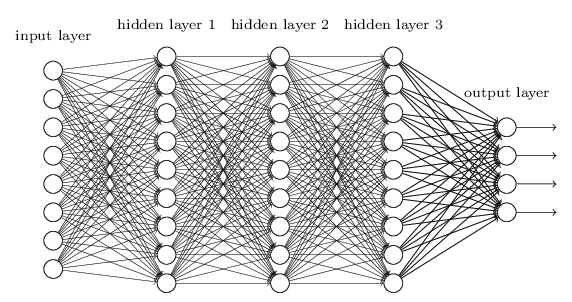
\includegraphics[width=1\linewidth]{../diagrams/decision-trees/neural}
	
	\label{fig:neural}
\end{figure}
\end{frame}

\begin{frame}{Learnt Decision Tree}
\begin{tikzpicture}[
node/.style={%
	draw,
	rectangle,
},
]

\node [node] (A) {Outlook};
\path (A) ++(-150:\nodeDist) node [node] (B) {Humidity};
\path (A) ++(-90:\nodeDist/2) node [node, fill=green] (C) {Yes};
\path (A) ++(-30:\nodeDist) node [node] (D) {Wind};
\path (B) ++(-135:\nodeDist) node [node, fill=red] (E) {No};
\path (B) ++(-45:\nodeDist) node [node, fill=green] (F) {Yes};
\path (D) ++(-45:\nodeDist) node [node, fill=red] (G) {No};
\path (D) ++(-135:\nodeDist) node [node, fill=green] (H) {Yes};

\draw (A) -- (B) node [left,pos=0.25] {Sunny}(A);
\draw (A) -- (C) node [right,pos=0.8] {Overcast}(A);
\draw (A) -- (D) node [right,pos=0.5] {Rain}(A);
\draw (B) -- (E) node [left,pos=0.25] {High}(A);
\draw (B) -- (F) node [right,pos=0.25] {Normal}(C);
\draw (D) -- (G) node [right,pos=0.25] {Strong}(A);
\draw (D) -- (H) node [left,pos=0.25] {Weak}(A);
\end{tikzpicture}

\end{frame}

\begin{frame}{Medical Diagnosis using Decision Trees }
\begin{figure}
	\centering
	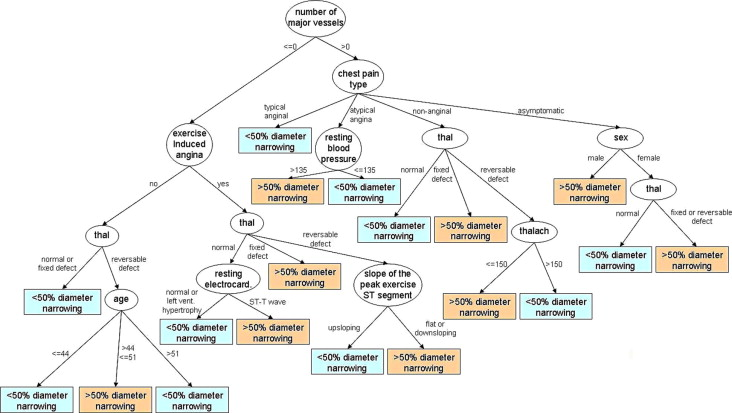
\includegraphics[width=1\linewidth]{../diagrams/decision-trees/decision-medical}
	\caption{Source: Improving medical decision trees by combining relevant health-care criteria}
	\label{fig:decision-medical}
\end{figure}

\end{frame}


\begin{frame}{Leo Brieman}
\begin{figure}
	\centering
	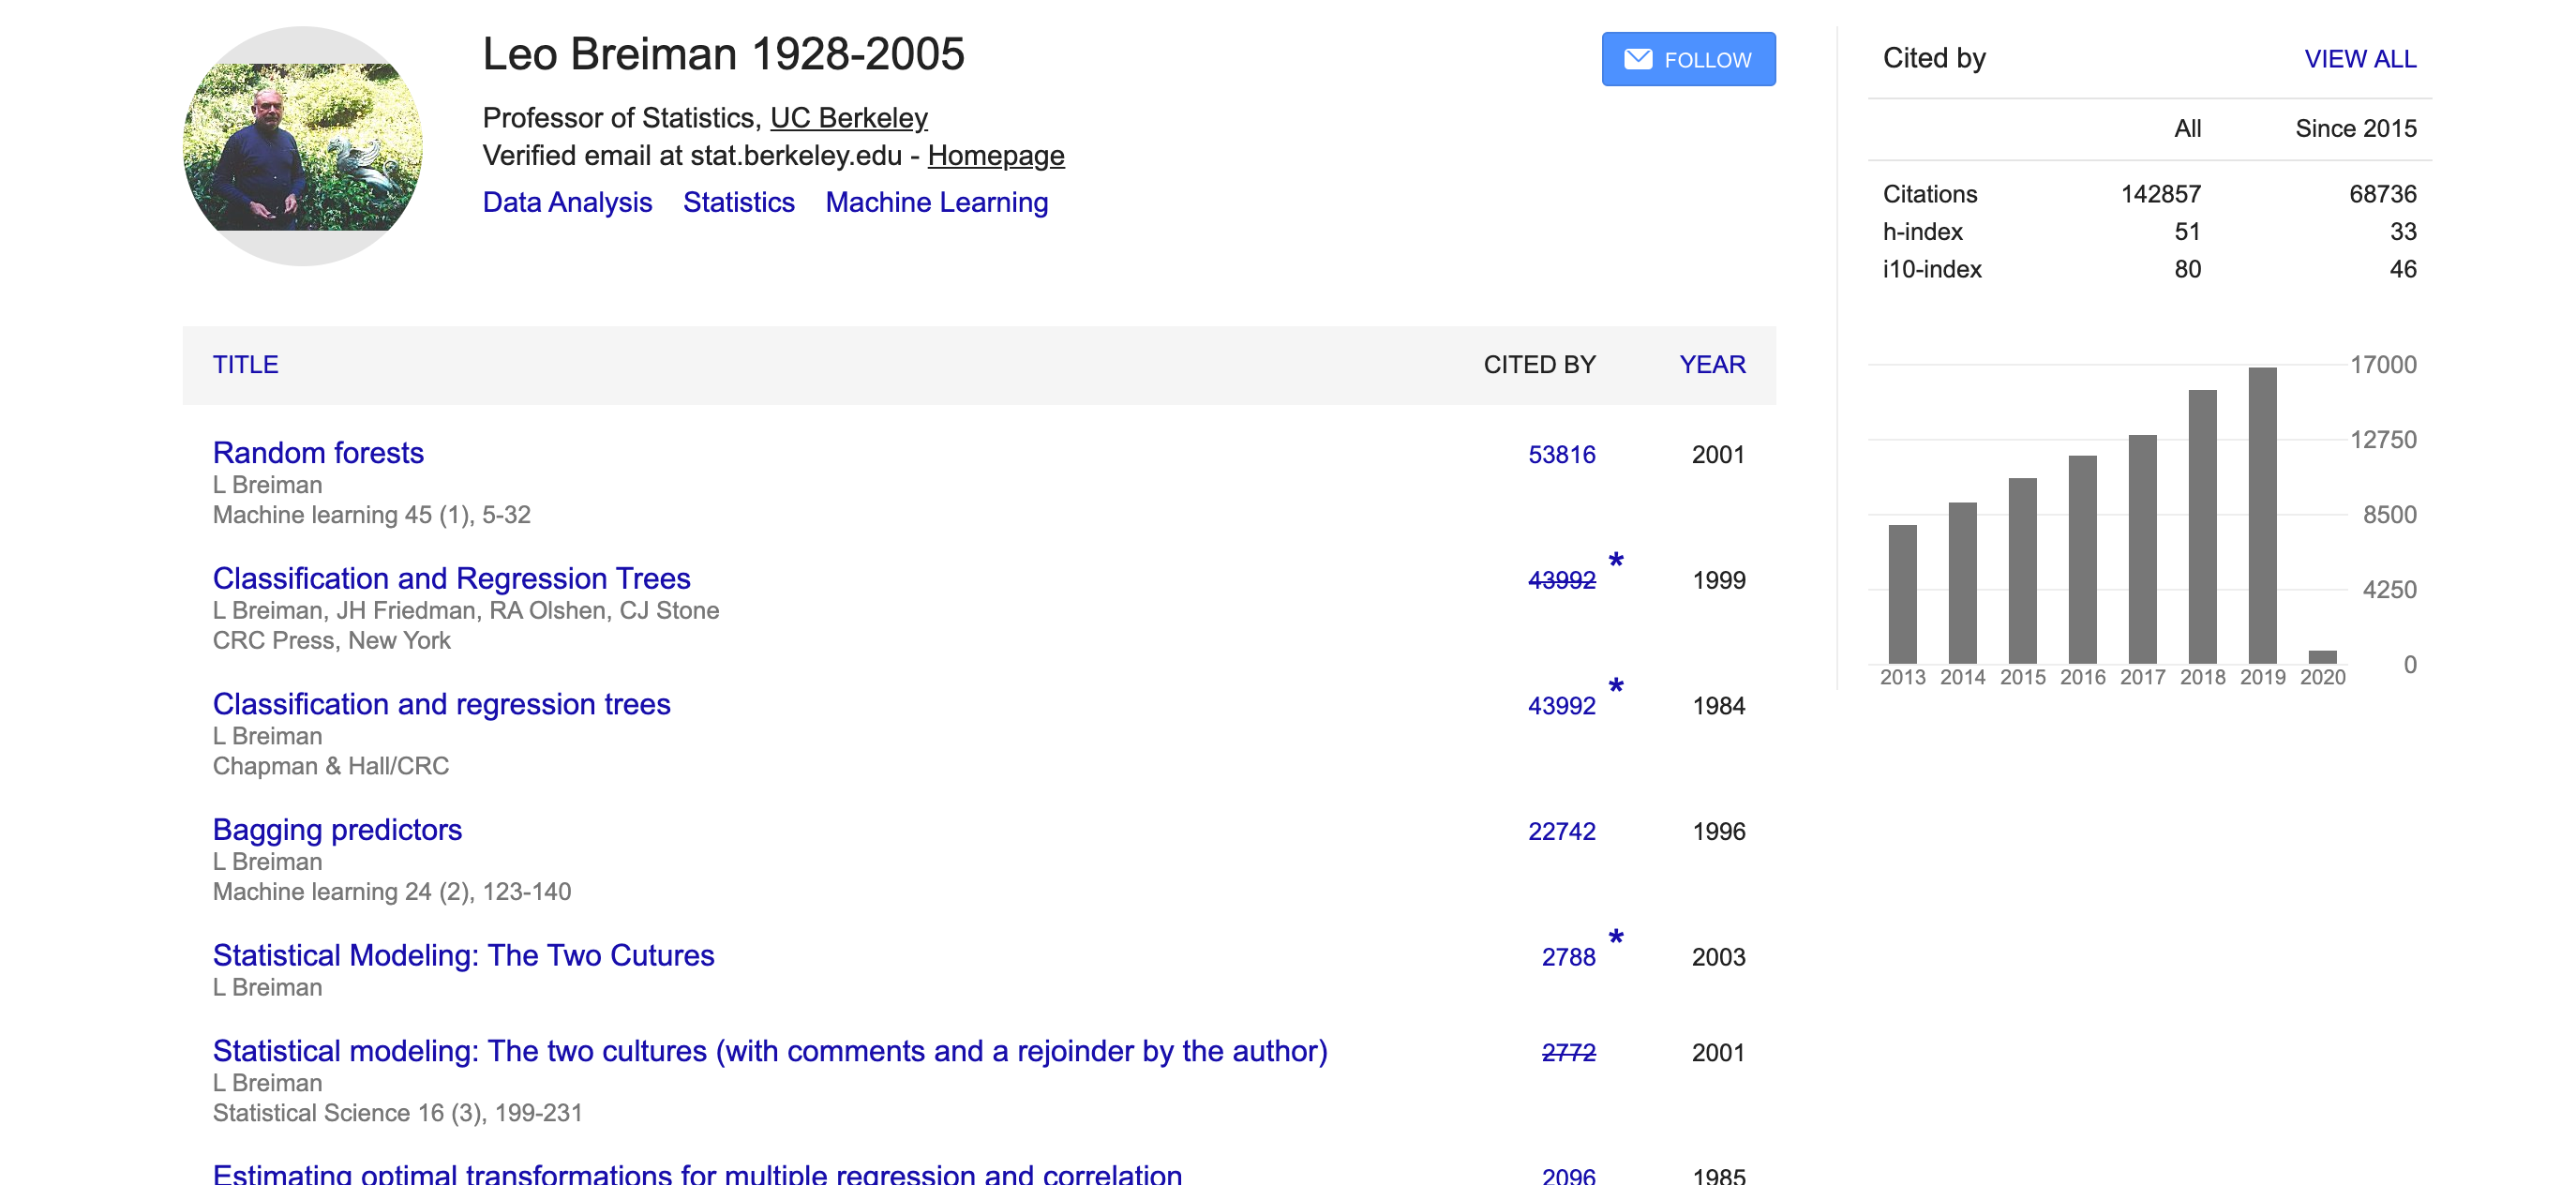
\includegraphics[width=1\linewidth]{../diagrams/decision-trees/brieman}

	\label{fig:brieman}
\end{figure}

\end{frame}

\begin{frame}{Optimal Decision Tree}
\begin{figure}
	\centering
	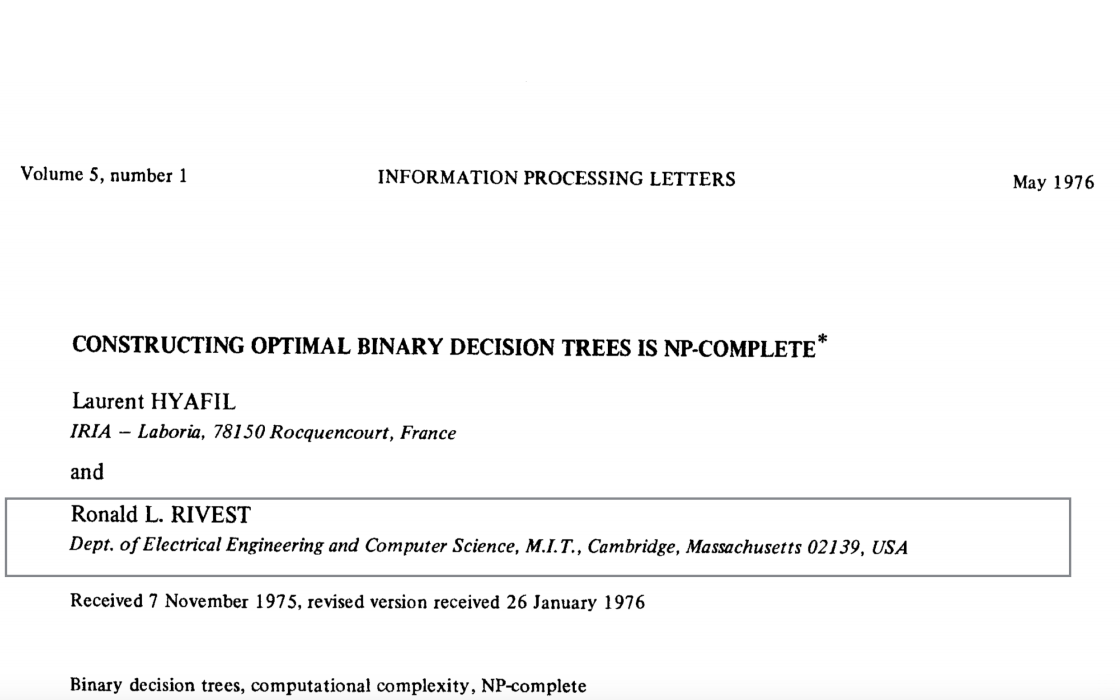
\includegraphics[width=1\linewidth]{../diagrams/decision-trees/NP-hard}

	\label{fig:np-hard}
\end{figure}

\end{frame}

\begin{frame}{Greedy Algorithm}
Core idea: At each level, choose an attribute that gives
\textbf{biggest estimated} performance gain!

\begin{figure}
	\centering
	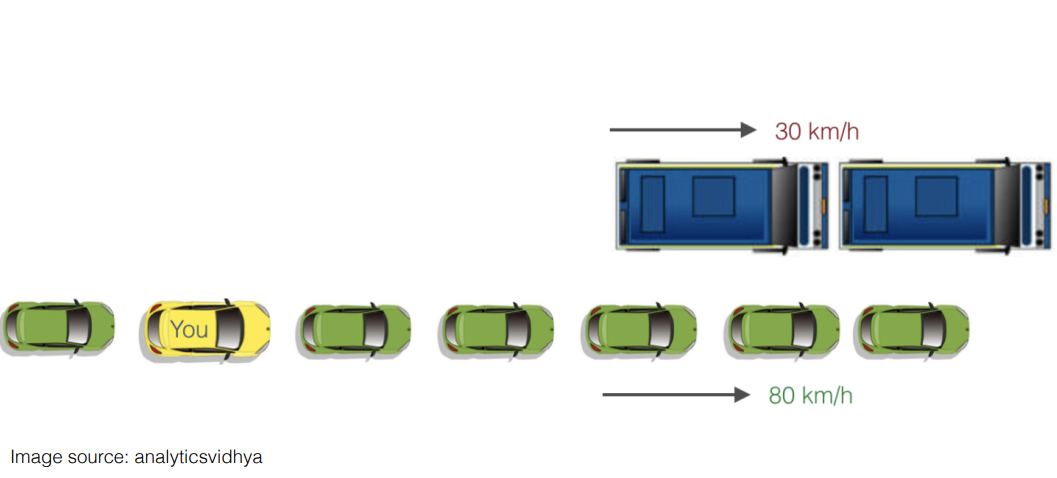
\includegraphics[width=0.8\linewidth]{../diagrams/decision-trees/gredy}
	\caption{Greedy!=Optimal}
	\label{fig:gredy}
\end{figure}

\end{frame}

\begin{frame}{Towards biggest estimated performance gain}
\begin{columns}
\begin{column}{.7\textwidth}


\begin{scriptsize}


	\begin{tabular}{lllll||l} \toprule
	\textbf{Day} & \textbf{Outlook}  & \textbf{Temp} & \textbf{Humidity} & \textbf{Windy}  & \textbf{Play} \\ \midrule
	D1  & Sunny    & Hot  & High     & Weak   & No   \\
	D2  & Sunny    & Hot  & High     & Strong & No   \\
	D3  & Overcast & Hot  & High     & Weak   & Yes  \\
	D4  & Rain     & Mild & High     & Weak   & Yes  \\
	D5  & Rain     & Cool & Normal   & Weak   & Yes  \\
	D6  & Rain     & Cool & Normal   & Strong & No   \\
	D7  & Overcast & Cool & Normal   & Strong & Yes  \\
	D8  & Sunny    & Mild & High     & Weak   & No   \\
	D9  & Sunny    & Cool & Normal   & Weak   & Yes  \\
	D10 & Rain     & Mild & Normal   & Weak   & Yes  \\
	D11 & Sunny    & Mild & Normal   & Strong & Yes  \\
	D12 & Overcast & Mild & High     & Strong & Yes  \\
	D13 & Overcast & Hot  & Normal   & Weak   & Yes  \\
	D14 & Rain     & Mild & High     & Strong & No  \\ \bottomrule
\end{tabular}
\end{scriptsize}
\end{column}
\begin{column}{0.4\textwidth}
	\begin{scriptsize}
\begin{itemize}
	\pause \item For examples, we have 9 Yes, 5 No
	\pause \item Would it be trivial if we had 14 Yes or 14 No?
	\pause \item Yes!
	\pause \item Key insights:  Problem is ``easier'' when there is lesser disagreement
	\pause 	\item Need some statistical measure of ``disagreement'' 
	\end{itemize}

\end{scriptsize}
\end{column}

\end{columns}

\end{frame}




%\begin{frame}
%\begin{forest}
%	for tree={grow'=south}
%	[Outlook
%	[Humidity, edge label={node[midway,fill=gray,font=\scriptsize]{Sunny}} []]
%	[Wind, edge label={node[midway,fill=white,font=\scriptsize]{Rain}} [] [] []]
%	[Yes, edge label={node[midway,fill=white,font=\scriptsize]{Overcast}}]
%	]
%\end{forest}
%\end{frame}

\begin{frame}{Entropy}
 Statistical measure to characterize the
(im)purity of examples

\pause $H(X) = -\sum_{i=1}^n p(x_i) \log p(x_i)$

\begin{figure}[htp]
    \centering
    \begin{notebookbox}{https://nipunbatra.github.io/ml-teaching/notebooks/entropy.html}
      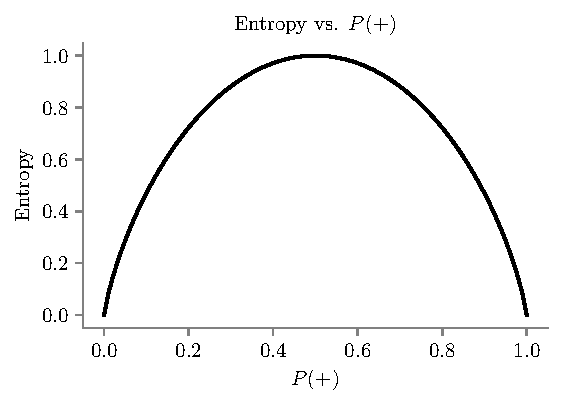
\includegraphics[width=0.7\linewidth]{../figures/decision-trees/entropy.pdf}
    \end{notebookbox}
  \end{figure}

\end{frame}
	
\begin{frame}{Towards biggest estimated performance gain}
\begin{columns}
	\begin{column}{.7\textwidth}
		
		
		\begin{scriptsize}
			

			\begin{tabular}{lllll||l} \toprule
				\textbf{Day} & \textbf{Outlook}  & \textbf{Temp} & \textbf{Humidity} & \textbf{Windy}  & \textbf{Play} \\ \midrule
				D1  & Sunny    & Hot  & High     & Weak   & No   \\
				D2  & Sunny    & Hot  & High     & Strong & No   \\
				D3  & Overcast & Hot  & High     & Weak   & Yes  \\
				D4  & Rain     & Mild & High     & Weak   & Yes  \\
				D5  & Rain     & Cool & Normal   & Weak   & Yes  \\
				D6  & Rain     & Cool & Normal   & Strong & No   \\
				D7  & Overcast & Cool & Normal   & Strong & Yes  \\
				D8  & Sunny    & Mild & High     & Weak   & No   \\
				D9  & Sunny    & Cool & Normal   & Weak   & Yes  \\
				D10 & Rain     & Mild & Normal   & Weak   & Yes  \\
				D11 & Sunny    & Mild & Normal   & Strong & Yes  \\
				D12 & Overcast & Mild & High     & Strong & Yes  \\
				D13 & Overcast & Hot  & Normal   & Weak   & Yes  \\
				D14 & Rain     & Mild & High     & Strong & No  \\ \bottomrule
			\end{tabular}
		\end{scriptsize}
	\end{column}
	\begin{column}{0.4\textwidth}
		\begin{scriptsize}
			\begin{itemize}
				\pause \item Can we use Outlook as the root node?
				\pause 	\item When Outlook is overcast, we always Play and thus no ``disagreement'' 
			\end{itemize}
			
		\end{scriptsize}
	\end{column}
	
\end{columns}

\end{frame}
	
\begin{frame}{Information Gain}
 Reduction in entropy
by partitioning examples (S) on attribute A
$$
\operatorname{Gain}(S, A) \equiv \text { Entropy }(S)-\sum_{v \in V a l u e s(A)} \frac{\left|S_{v}\right|}{|S|} \text {Entropy}\left(S_{v}\right)
$$
\end{frame}


\begin{frame}{ID3 (Examples, Target Attribute, Attributes)}
\begin{itemize}[<+->]
	\item Create a root node for tree
	\item If all examples are +/-, return root with label = +/-
	\item  If attributes = empty, return root with most common value of
	Target Attribute in Examples
	\item Begin
	\begin{itemize}[<+->]
		\item A $\leftarrow$ attribute from Attributes which best classifies
		Examples
		\item 	Root $\leftarrow$ A
		\item  For each value (v) of A
		\begin{itemize}[<+->]
			\item Add new tree branch : A = v
			\item  Examples\textsubscript{v}: subset of examples that A = v
			\item If Examples\textsubscript{v}is empty: add leaf with label = most
			common value of Target Attribute
			\item Else: ID3 (Examples\textsubscript{v}, Target attribute, Attributes - {A})
		\end{itemize}
	\end{itemize}


\end{itemize}
\end{frame}

\begin{frame}{Learnt Decision Tree}
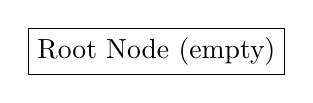
\begin{tikzpicture}[
node/.style={%
	draw,
	rectangle,
},
]

\node [node] (A) {Root Node (empty)};

\end{tikzpicture}

\end{frame}

	\begin{frame}{Training Data}
\begin{tabular}{lllll||l} \toprule
	\textbf{Day} & \textbf{Outlook}  & \textbf{Temp} & \textbf{Humidity} & \textbf{Windy}  & \textbf{Play} \\ \midrule
	D1  & Sunny    & Hot  & High     & Weak   & No   \\
	D2  & Sunny    & Hot  & High     & Strong & No   \\
	D3  & Overcast & Hot  & High     & Weak   & Yes  \\
	D4  & Rain     & Mild & High     & Weak   & Yes  \\
	D5  & Rain     & Cool & Normal   & Weak   & Yes  \\
	D6  & Rain     & Cool & Normal   & Strong & No   \\
	D7  & Overcast & Cool & Normal   & Strong & Yes  \\
	D8  & Sunny    & Mild & High     & Weak   & No   \\
	D9  & Sunny    & Cool & Normal   & Weak   & Yes  \\
	D10 & Rain     & Mild & Normal   & Weak   & Yes  \\
	D11 & Sunny    & Mild & Normal   & Strong & Yes  \\
	D12 & Overcast & Mild & High     & Strong & Yes  \\
	D13 & Overcast & Hot  & Normal   & Weak   & Yes  \\
	D14 & Rain     & Mild & High     & Strong & No  \\ \bottomrule
\end{tabular}
\end{frame}


\begin{frame}{Entropy calculated}
We have 14 examples in $S$: 5 No, 9 Yes

$$\operatorname{Entropy(S)} = -\operatorname{p}_{No}\operatorname{log_2}{\operatorname{p}_{No}}
-\operatorname{p}_{Yes}\operatorname{log_2}{\operatorname{p}_{Yes}}$$
$$
=-(5 / 14) \log _{2}(5 / 14)-(9 / 14) \log _{2}(9 / 14) =0.94
$$
\end{frame}

\begin{frame}{Information Gain for Outlook}
\begin{tabular}{l|l} \toprule
\textbf{Outlook} & \textbf{Play} \\ \midrule
Sunny    & No   \\
Sunny    & No   \\
Overcast & Yes  \\
Rain     & Yes  \\
Rain     & Yes  \\
Rain     & No   \\
Overcast & Yes  \\
Sunny    & No   \\
Sunny    & Yes  \\
Rain     & Yes  \\
Sunny    & Yes  \\
Overcast & Yes  \\
Overcast & Yes  \\
Rain     & No  \\ \bottomrule
\end{tabular}
\end{frame}

\begin{frame}{Information Gain for Outlook}
\begin{columns}


\begin{column}{.32\textwidth}
	\begin{table}
\begin{tabular}{l|l} \toprule
	\textbf{Outlook} & \textbf{Play} \\ \midrule
	Sunny    & No   \\
	Sunny    & No   \\
	Sunny    & No   \\
	Sunny    & Yes  \\
	Sunny    & Yes  \\

\bottomrule
\end{tabular}
We have 2 Yes, 3 No
Entropy = (-3/5)$\log_{2}$(3/5) - (-2/5)$\log_{2}$(2/5) = 0.971
\end{table}
\end{column}

\pause \begin{column}{.32\textwidth}
	\begin{table}


\begin{tabular}{l|l} \toprule
	\textbf{Outlook} & \textbf{Play} \\ \midrule

	Overcast & Yes  \\
	Overcast & Yes  \\
	Overcast & Yes  \\
	Overcast & Yes  \\ \bottomrule

\end{tabular}
We have 4 Yes, 0 No
Entropy = 0


	\end{table}


\end{column}


\pause \begin{column}{.32\textwidth}
	\begin{table}
\begin{tabular}{l|l} \toprule
	\textbf{Outlook} & \textbf{Play} \\ \midrule
	Rain     & Yes  \\
	Rain     & Yes  \\
	Rain     & No   \\
	Rain     & Yes  \\
	Rain     & No  \\ \bottomrule
\end{tabular}
We have 3 Yes, 2 No
Entropy = (-3/5)$\log_{2}$(3/5) - (-2/5)$\log_{2}$(2/5) = 0.971
\end{table}
\end{column}
\end{columns}
\end{frame}

\begin{frame}{Information Gain}
$$
\operatorname{Gain}(S, Outlook) = \text { Entropy }(S)-\sum_{v \in \{Rain, Sunny, Windy\}} \frac{\left|S_{v}\right|}{|S|} \text {Entropy}\left(S_{v}\right) 
$$

Gain (S, Outlook) $=$ Entropy $(\mathrm{S})$ -$(5 / 14)$* Entropy(S\textsubscript{Sunny})- $(4 / 14)$* Entropy (S\textsubscript{overcast})$-(5 / 14)$* Entropy(S\textsubscript{Rain}) \\

= 0.940 - 0.347 - 0.347 \\
= 0.246

\end{frame}

\begin{frame}{Information Gain}


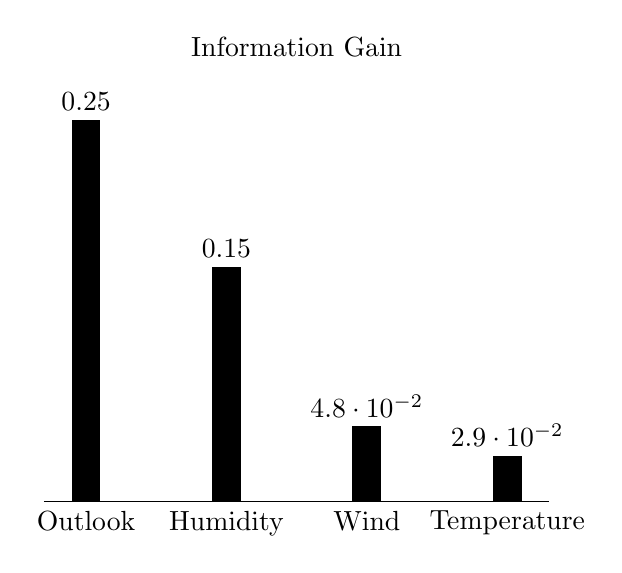
\begin{tikzpicture}
\begin{axis}[
symbolic x coords={Outlook,Humidity,Wind,Temperature},
xtick=data,xtick pos=left, width=8cm,
ytick pos=left,axis x line*=bottom,nodes near coords,hide y axis,title=Information Gain, ymin=0.0]
\addplot[ybar,fill=black] coordinates {
	(Outlook,0.246)
	(Humidity,0.151)
	(Wind,0.048)
	(Temperature,0.029)
};
\end{axis}
\end{tikzpicture}


\end{frame}

\begin{frame}{Learnt Decision Tree}
\begin{tikzpicture}[
node/.style={%
	draw,
	rectangle,
},
]

\node [node] (A) {Outlook};
\path (A) ++(-150:\nodeDist) node [node] (B) {?};
\path (A) ++(-90:\nodeDist/2) node [node, fill=green] (C) {Yes};
\path (A) ++(-30:\nodeDist) node [node] (D) {?};


\draw (A) -- (B) node [left,pos=0.25] {Sunny}(A);
\draw (A) -- (C) node [right,pos=0.8] {Overcast}(A);
\draw (A) -- (D) node [right,pos=0.5] {Rain}(A);

\end{tikzpicture}

\end{frame}

	\begin{frame}{Calling ID3 on Outlook=Sunny}
\begin{tabular}{llll||l} \toprule
	\textbf{Day} & \textbf{Temp} & \textbf{Humidity} & \textbf{Windy}  & \textbf{Play} \\ \midrule
	D1    & Hot  & High     & Weak   & No   \\
	D2     & Hot  & High     & Strong & No   \\
	D8     & Mild & High     & Weak   & No   \\
	D9    & Cool & Normal   & Weak   & Yes  \\
	D11    & Mild & Normal   & Strong & Yes  \\ \bottomrule
\end{tabular}

\begin{itemize}
	\pause \item Gain(S\textsubscript{Outlook=Sunny}, Temp) = Entropy(3 Yes, 2 No) - (2/5)*Entropy(2 No, 0 Yes) -(2/5)*Entropy(1 No, 1 Yes) - (1/5)*Entropy(1 Yes) 
	\pause \item Gain(S\textsubscript{Outlook=Sunny}, Humidity) = Entropy(3 Yes, 2 No) - (2/5)*Entropy(2 Yes) -(3/5)*Entropy(3 No) $\implies$ \textbf{maximum possible for the set}
	\pause \item Gain(S\textsubscript{Outlook=Sunny}, Windy) = Entropy(3 Yes, 2 No) - (3/5)*Entropy(2 No, 1 Yes) -(2/5)*Entropy(1 No, 1 Yes) 
\end{itemize}
\end{frame}

\begin{frame}{Learnt Decision Tree}
\begin{tikzpicture}[
node/.style={%
	draw,
	rectangle,
},
]

\node [node] (A) {Outlook};
\path (A) ++(-150:\nodeDist) node [node] (B) {Humidity};
\path (A) ++(-90:\nodeDist/2) node [node, fill=green] (C) {Yes};
\path (A) ++(-30:\nodeDist) node [node] (D) {?};
\path (B) ++(-135:\nodeDist) node [node, fill=red] (E) {No};
\path (B) ++(-45:\nodeDist) node [node, fill=green] (F) {Yes};
;

\draw (A) -- (B) node [left,pos=0.25] {Sunny}(A);
\draw (A) -- (C) node [right,pos=0.8] {Overcast}(A);
\draw (A) -- (D) node [right,pos=0.5] {Rain}(A);
\draw (B) -- (E) node [left,pos=0.25] {High}(A);
\draw (B) -- (F) node [right,pos=0.25] {Normal}(C);

\end{tikzpicture}

\end{frame}


	\begin{frame}{Calling ID3 on (Outlook=Rain)}
\begin{tabular}{llll||l} \toprule
	\textbf{Day}  & \textbf{Temp} & \textbf{Humidity} & \textbf{Windy}  & \textbf{Play} \\ \midrule
	D4    & Mild & High     & Weak   & Yes  \\
	D5     & Cool & Normal   & Weak   & Yes  \\
	D6      & Cool & Normal   & Strong & No   \\
	D10     & Mild & Normal   & Weak   & Yes  \\
	D14      & Mild & High     & Strong & No  \\ \bottomrule
\end{tabular}
\begin{itemize}
	\item The attribute Windy gives the highest information gain
\end{itemize}
\end{frame}

\begin{frame}{Learnt Decision Tree}
\begin{tikzpicture}[
node/.style={%
	draw,
	rectangle,
},
]

\node [node] (A) {Outlook};
\path (A) ++(-150:\nodeDist) node [node] (B) {Humidity};
\path (A) ++(-90:\nodeDist/2) node [node, fill=green] (C) {Yes};
\path (A) ++(-30:\nodeDist) node [node] (D) {Wind};
\path (B) ++(-135:\nodeDist) node [node, fill=red] (E) {No};
\path (B) ++(-45:\nodeDist) node [node, fill=green] (F) {Yes};
\path (D) ++(-45:\nodeDist) node [node, fill=red] (G) {No};
\path (D) ++(-135:\nodeDist) node [node, fill=green] (H) {Yes};

\draw (A) -- (B) node [left,pos=0.25] {Sunny}(A);
\draw (A) -- (C) node [right,pos=0.8] {Overcast}(A);
\draw (A) -- (D) node [right,pos=0.5] {Rain}(A);
\draw (B) -- (E) node [left,pos=0.25] {High}(A);
\draw (B) -- (F) node [right,pos=0.25] {Normal}(C);
\draw (D) -- (G) node [right,pos=0.25] {Strong}(A);
\draw (D) -- (H) node [left,pos=0.25] {Weak}(A);
\end{tikzpicture}

\end{frame}

\begin{frame}{Prediction for Decision Tree}
Just walk down the tree!

\begin{tikzpicture}[
node/.style={%
	draw,
	rectangle,
},
]

\node [node] (A) {Outlook};
\path (A) ++(-150:\nodeDist) node [node] (B) {Humidity};
\path (A) ++(-90:\nodeDist/2) node [node, fill=green] (C) {Yes};
\path (A) ++(-30:\nodeDist) node [node] (D) {Wind};
\path (B) ++(-135:\nodeDist) node [node, fill=red] (E) {No};
\path (B) ++(-45:\nodeDist) node [node, fill=green] (F) {Yes};
\path (D) ++(-45:\nodeDist) node [node, fill=red] (G) {No};
\path (D) ++(-135:\nodeDist) node [node, fill=green] (H) {Yes};

\draw (A) -- (B) node [left,pos=0.25] {Sunny}(A);
\draw (A) -- (C) node [right,pos=0.8] {Overcast}(A);
\draw (A) -- (D) node [right,pos=0.5] {Rain}(A);
\draw (B) -- (E) node [left,pos=0.25] {High}(A);
\draw (B) -- (F) node [right,pos=0.25] {Normal}(C);
\draw (D) -- (G) node [right,pos=0.25] {Strong}(A);
\draw (D) -- (H) node [left,pos=0.25] {Weak}(A);
\end{tikzpicture}

\pause Prediction for $<$High Humidity, Strong Wind, Sunny Outlook, Hot Temp$>$ is ? \\
\pause  No
\end{frame}

\begin{frame}{Limiting Depth of Tree}
Assuming if you were only allowed depth-$1$ trees, how would it look for the current dataset? \\

\pause Apply the same rules, except when depth limit reached, the leaf node is assigned the ``most'' common occuring value in that path.

\pause What is depth-$0$ tree (no decision) for the examples? \\
\pause Always predicting Yes

\pause What is depth-$1$ tree (no decision) for the examples? \\
\pause \begin{tikzpicture}[
node/.style={%
	draw,
	rectangle,
},
]

\node [node] (A) {Outlook};
\path (A) ++(-150:\nodeDist) node [node, fill=red] (B) {No};
\path (A) ++(-90:\nodeDist/2) node [node, fill=green] (C) {Yes};
\path (A) ++(-30:\nodeDist) node [node, fill=green] (D) {Yes};


\draw (A) -- (B) node [left,pos=0.25] {Sunny}(A);
\draw (A) -- (C) node [right,pos=0.8] {Overcast}(A);
\draw (A) -- (D) node [right,pos=0.5] {Rain}(A);

\end{tikzpicture}

\end{frame}

\section{Discrete Input, Real Output}

\begin{frame}{Modified Dataset}
\begin{table}[]
	\begin{tabular}{@{}llllll@{}}
		\toprule
		\textbf{Day} & \textbf{Outlook} & \textbf{Temp} & \textbf{Humidity} & \textbf{Wind} & \textbf{Minutes Played} \\ \midrule
		D1           & Sunny            & Hot           & High              & Weak          & 20                      \\
		D2           & Sunny            & Hot           & High              & Strong        & 24                      \\
		D3           & Overcast         & Hot           & High              & Weak          & 40                      \\
		D4           & Rain             & Mild          & High              & Weak          & 50                      \\
		D5           & Rain             & Cool          & Normal            & Weak          & 60                      \\
		D6           & Rain             & Cool          & Normal            & Strong        & 10                      \\
		D7           & Overcast         & Cool          & Normal            & Strong        & 4                       \\
		D8           & Sunny            & Mild          & High              & Weak          & 10                      \\
		D9           & Sunny            & Cool          & Normal            & Weak          & 60                      \\
		D10          & Rain             & Mild          & Normal            & Weak          & 40                      \\
		D11          & Sunny            & Mild          & High              & Strong        & 45                      \\
		D12          & Overcast         & Mild          & High              & Strong        & 40                      \\
		D13          & Overcast         & Hot           & Normal            & Weak          & 35                      \\
		D14          & Rain             & Mild          & High              & Strong        & 20                      \\ \bottomrule
	\end{tabular}
\end{table}
\end{frame}

\begin{frame}{Measure of Impurity for Regression?}
\begin{itemize}
	\item \pause Any guesses?
	\item \pause Mean Squared Error
	\item \pause MSE(S) = 311.34
	\item \pause Information Gain analogoue?
	\item \pause Reduction in MSE (weighted)
\end{itemize}

\end{frame}

\begin{frame}{Gain by splitting on Wind}
\begin{columns}

\begin{column}{.5\textwidth}
	\begin{scriptsize}

\begin{table}[]
	\begin{tabular}{@{}ll@{}}
		\toprule
		\textbf{Wind} & \textbf{Minutes Played} \\ \midrule
		Weak          & 20                      \\
		Strong        & 24                      \\
		Weak          & 40                      \\
		Weak          & 50                      \\
		Weak          & 60                      \\
		Strong        & 10                      \\
		Strong        & 4                       \\
		Weak          & 10                      \\
		Weak          & 60                      \\
		Weak          & 40                      \\
		Strong        & 45                      \\
		Strong        & 40                      \\
		Weak          & 35                      \\
		Strong        & 20                      \\ \bottomrule
	\end{tabular}
\caption{MSE(S)=311.34}
\end{table}
	\end{scriptsize}
\end{column}
\begin{column}{.5\textwidth}
	\begin{tiny}
\vspace{-5pt}		
\begin{table}[]
	\begin{tabular}{@{}ll@{}}
		\toprule
		\textbf{Wind} & \textbf{Minutes Played} \\ \midrule
		Weak          & 20                      \\
		Weak          & 40                      \\
		Weak          & 50                      \\
		Weak          & 60                      \\
		Weak          & 10                      \\
		Weak          & 60                      \\
		Weak          & 40                      \\
		Weak          & 35                      \\ \bottomrule
	\end{tabular}
\caption{Weighted MSE(S\textsubscript{Wind=Weak}=(8/14)*277=159)}
\end{table}
\vspace{-25pt}
	\end{tiny}

	\begin{tiny}
	
	\begin{table}[]
		\begin{tabular}{@{}ll@{}}
			\toprule
			\textbf{Wind} & \textbf{Minutes Played} \\ \midrule

			Strong        & 24                      \\
			Strong        & 10                      \\
			Strong        & 4                       \\
			Strong        & 45                      \\
			Strong        & 40                      \\
			Strong        & 20                      \\ \bottomrule
		\end{tabular}
\caption{Weighted MSE(S\textsubscript{Wind=Strong}=(6/14)*218=93)}
	\end{table}
\end{tiny}

\end{column}
\end{columns}
\end{frame}






\begin{frame}{Information Gain}

	\begin{figure}[htp]
		\centering
		\begin{notebookbox}{https://nipunbatra.github.io/ml-teaching/notebooks/decision-tree-real-output.html}
		  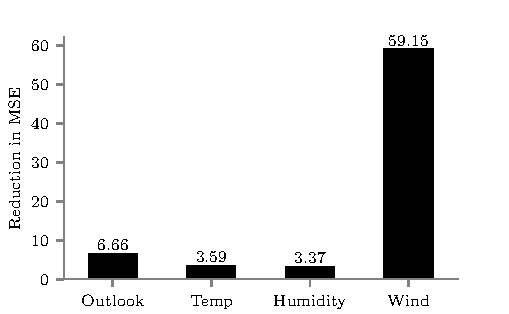
\includegraphics[width=\linewidth]{../figures/decision-trees/discrete-input-real-output-level-1.pdf}
		\end{notebookbox}
	  \end{figure}

\end{frame}

\begin{frame}{Learnt Tree}
\begin{figure}
	\centering
	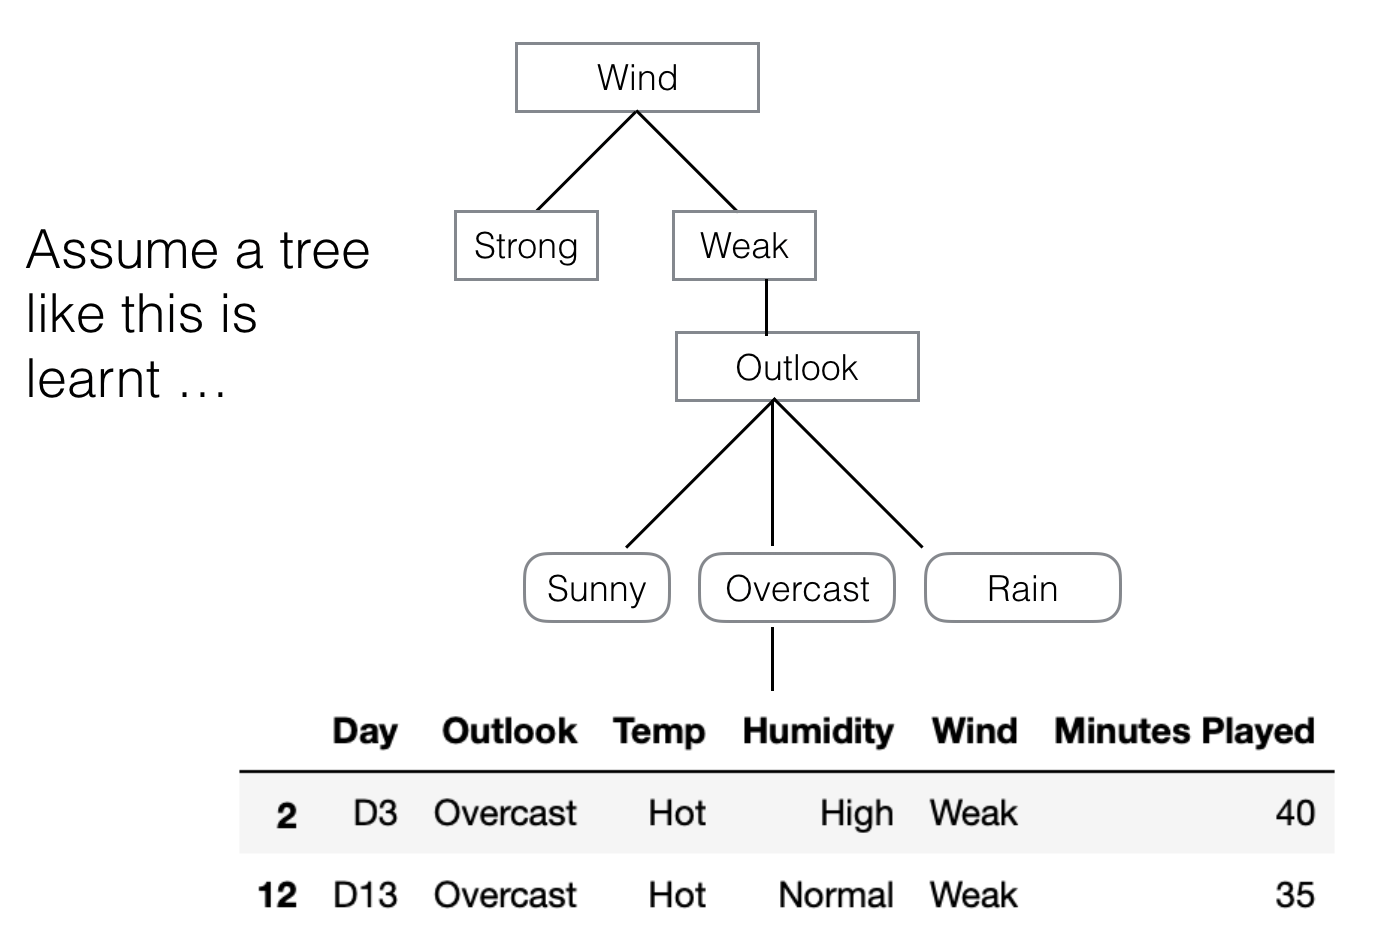
\includegraphics[width=1\linewidth]{../diagrams/decision-trees/tree}

	\label{fig:tree}
\end{figure}

\end{frame}

\begin{frame}{Learnt Tree}
\begin{figure}
	\centering
	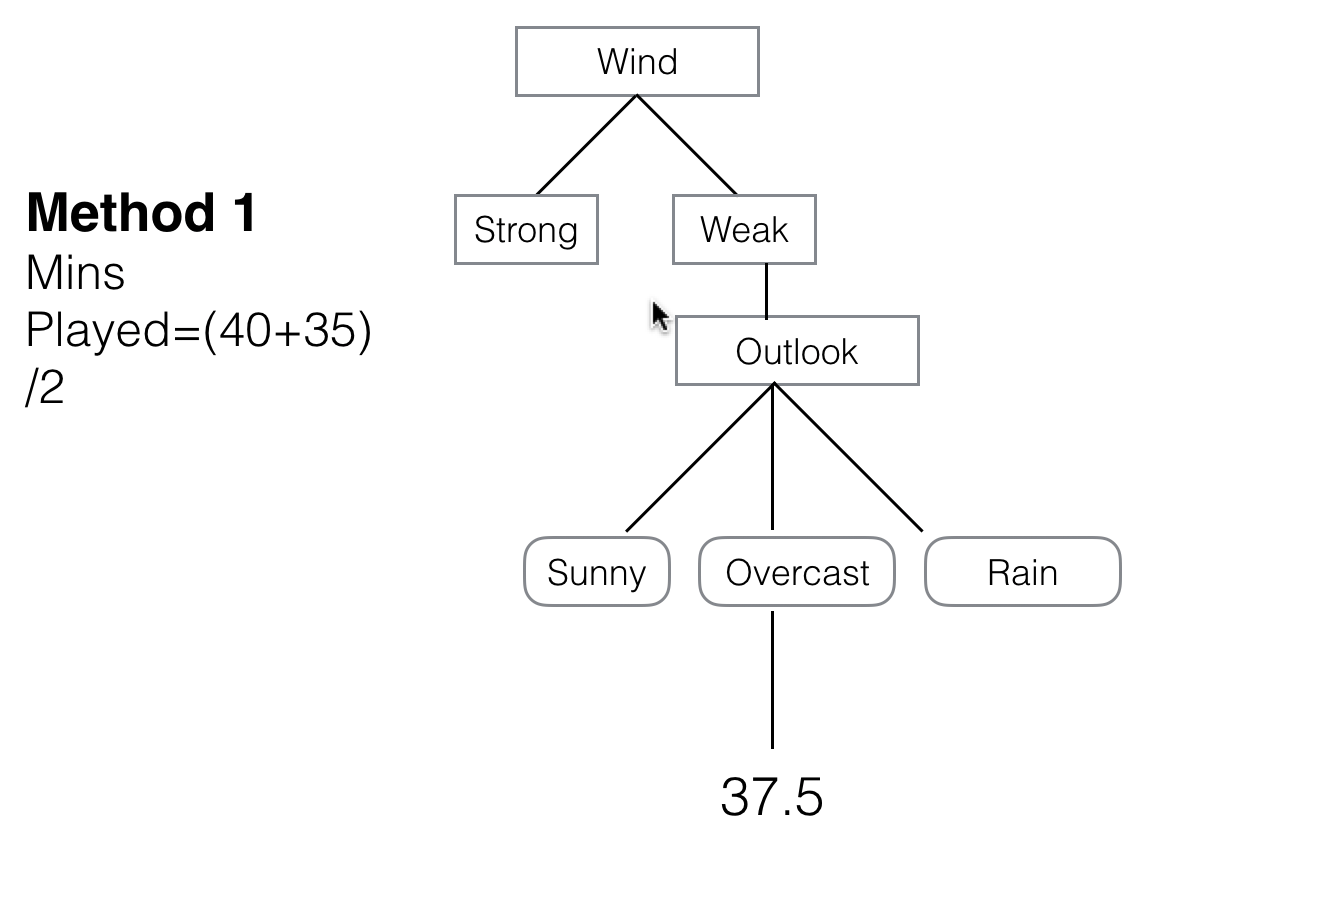
\includegraphics[width=1\linewidth]{../diagrams/decision-trees/tree2}

	\label{fig:tree}
\end{figure}

\end{frame}

\section{Real Input Discrete Output}


\begin{frame}{Finding splits}
\begin{table}[]
	\begin{tabular}{@{}lrr@{}}
		\toprule
		\textbf{Day} & \textbf{Temperature} & \textbf{PlayTennis} \\ \midrule
		D1           & 40                   & No                  \\
		D2           & 48                   & No                  \\
		D3           & 60                   & Yes                 \\
		D4           & 72                   & Yes                 \\
		D5           & 80                   & Yes                 \\
		D6           & 90                   & No                  \\ \bottomrule
	\end{tabular}
\end{table}
\begin{itemize}
	\item How do you find splits?
	\item Sort by attribute
	\item Find attribute values where changes happen
	\item For example, splits are: Temp $>$ (48+60)/2 and Temp $>$ (80+90)/2
\end{itemize}
\end{frame}

\foreach \i in {0,...,9} {
\begin{frame}{Example (DT of depth \i)}
    \begin{figure}
        \centering
        \includegraphics[scale=0.5]{../figures/decision-trees/dt-\i.pdf}
            \label{fig:dt-\i}
        
    \end{figure}
\end{frame}
}








\end{document}